%% -------------------------------------------------------------------------------------
%% tcc-poster.tex -- MAIN FILE
%% -------------------------------------------------------------------------------------

% Based from example code found in
% http://www-i6.informatik.rwth-aachen.de/~dreuw/latexbeamerposter.php
%=========================================================================
\documentclass[final,brazil]{beamer}
\usepackage{grffile}
\mode<presentation>{\usetheme{I6dv}}
\usepackage[brazil]{babel}
\usepackage[utf8]{inputenc}
%\usepackage{amsmath,amsthm, amssymb, latexsym}
%\usepackage{times}\usefonttheme{professionalfonts}  % obsolete
%\usefonttheme[onlymath]{serif}
%\boldmath
\usepackage[orientation=landscape,size=a2,scale=1,debug]{beamerposter}
% change list indention level
% \setdefaultleftmargin{3em}{}{}{}{}{}

\usepackage{array,booktabs,tabularx}
\usepackage[unicode]{hyperref}

\usepackage{subcaption}         % \begin{subfigure}
\usepackage{wrapfig}            % \begin{wrapfigure}
\usepackage{blindtext}

% centered tabularx columns
\newcolumntype{Z}{>{\centering\arraybackslash}X}
% phantom introduces a vertical space in p formatted table columns??!!
\newcommand{\pphantom}{\textcolor{ta3aluminium}}

\newcommand{\mytilde}{\raise.17ex\hbox{$\scriptstyle\mathtt{\sim}$}}

\newcommand{\blockouterspace}{\vskip1ex}

\newenvironment{innercol}{
\begin{columns}
  \begin{column}{.93\textwidth}
    \justifying
}{
  \end{column}
\end{columns}
}

%%%%%%%%%%%%%%%%%%%%%%%%%%%%%%%%%%%%%%%%%%%%%%%%%%%%%%%%%%%%%%%%%%%%%%%%%%%%%%%%%%%%%%
\graphicspath{{figs/}}

\title{\huge Anatomia do BitTorrent: a Ciência da Computação por trás do protocolo}
\author{Paulo Cheadi Haddad Filho --- \,\mytilde paulochf}
\institute[Universidade de São Paulo]
{Orientador: José Coelho de Pina --- \,\mytilde coelho \hspace*{\;\;\qquad}}

%%%%%%%%%%%%%%%%%%%%%%%%%%%%%%%%%%%%%%%%%%%%%%%%%%%%%%%%%%%%%%%%%%%%%%%%%%%%%%%%%%%%%%
\newlength{\columnheight}
\setlength{\columnheight}{105cm}


%%%%%%%%%%%%%%%%%%%%%%%%%%%%%%%%%%%%%%%%%%%%%%%%%%%%%%%%%%%%%%%%%%%%%%%%%%%%%%%%%%%%%%
\begin{document}
\begin{frame}
  \begin{columns}
    % ---------------------------------------------------------%
    % Set up a column
    \begin{column}{.245\textwidth}
      \begin{beamercolorbox}[center,wd=\textwidth]{postercolumn}
        \begin{minipage}[T]{.95\textwidth}  % tweaks the width, makes a new \textwidth
          \parbox[t][\columnheight]{\textwidth}{ % must be some better way to set the the height, width and textwidth simultaneously
            % Since all columns are the same length, it is all nice and tidy.  You have to get the height empirically
            % ---------------------------------------------------------%
            % fill each column with content

            \begin{block}{Introdução}
              \begin{innercol}
                \begin{itemize}
                  \justifying
                  \item \textbf{redes \emph{peer-to-peer} (P2P)}: redes de arquitetura
                descentralizada (sem um servidor central) e distribuída entre vários
                nós da rede (\emph{peers})
                  \item \textbf{Napster} foi a primeira rede P2P, em 1999
                \end{itemize}
              \end{innercol}
            \end{block}

            \blockouterspace

            \begin{block}{História do BitTorrent}
              \begin{innercol}
                \begin{itemize}
                  \justifying
                  \item lançado por Bram Cohen em \textbf{2001}
                  \item protocolo P2P \textbf{mais usado no mundo}, que gera
                    $\approx \!\!\: 23 \%$ do tráfego de upload, $\approx \!\! 17 \%$ de
                    download e $\approx \!\! 10 \%$ de todo o tráfego na América Latina
                    \cite{sandvine}
                  \item usado por \textbf{Twitter} \cite{torrentfreak:twitter} e
                    \textbf{Facebook} \cite{torrentfreak:facebook} para distribuir
                    os códigos dos seus sites para seus servidores
                  \item baseado em \textbf{trocas justas} de arquivos e
                    \textbf{comunicação eficiente} entre \emph{peers}
                  \item peers \textbf{sugadores} (\emph{leechers}) e \textbf{semeadores}
                    (\emph{seeders}) trocam dados entre si
                  \item \textbf{listas de \emph{peers}} mantidas por
                    \textbf{rastreadores} (\emph{trackers}) e, geralmente, pelos
                    próprios \emph{peers}
                \end{itemize}
              \end{innercol}
            \end{block}

            \blockouterspace

            \begin{block}{Transmission}
              \begin{innercol}
                \begin{wrapfigure}{l}{.2\linewidth}
                  \vspace{-1ex}
                  \hspace{-1ex}
                  
\includegraphics[width=\linewidth]{transmission.png}
                \end{wrapfigure}

                \begin{itemize}
                  \justifying
                  \vspace{-4ex}
                  \item \textbf{programa cliente} de \textbf{código aberto} para o
                    protocolo BitTorrent
                  \item escrito nas linguagens \textbf{C} e \textbf{C++}
                  \item \textbf{várias plataformas}: \emph{daemon} (serviço de segundo
                    plano), roteadores, linha de comando e aplicação em janela
                \end{itemize}
              \end{innercol}
            \end{block}

            \blockouterspace

            \begin{block}{BitTorrent: visão do usuário e áreas da Computação}
              \begin{figure}
                \centering
                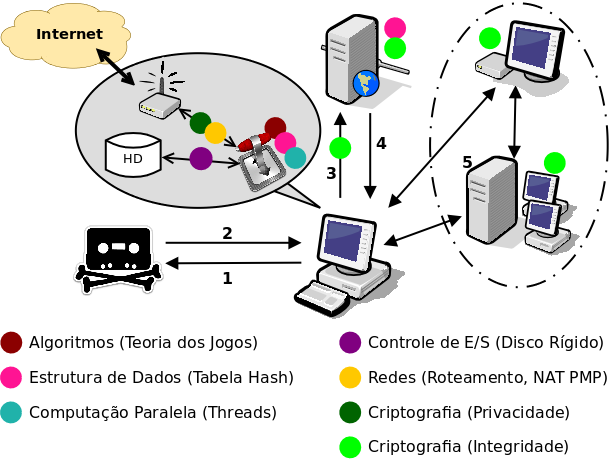
\includegraphics[width=\textwidth]{funcionamento.png}
              \end{figure}

              \begin{columns}
                \hspace{-6ex}
                \begin{column}{.97\textwidth}
                  \begin{enumerate}
                    % Enumerate não tá funcionando =P
                    \justifying
                    \item \textbf{1.} busca de conteúdo em sites buscadores de torrent
                    \item \textbf{2.} obtenção do arquivo .torrent desejado
                    \item \textbf{3.} computador do usuário se comunica com rastreadores
                      (\emph{trackers}), que mantêm listas dos \emph{peers} que estão
                      compartilhando os arquivos do torrent obtido
                    \item \textbf{4.} o \emph{tracker} devolve uma lista de \emph{peers}
                      aleatória
                    \item \textbf{5.} computador do usuário inicia comunicação com os
                      \emph{peers} da lista, e começa a receber deles os arquivos
                      pertencentes àquele torrent
                  \end{enumerate}
                \end{column}
              \end{columns}
            \end{block}
          }
        \end{minipage}
      \end{beamercolorbox}
    \end{column}
    % ---------------------------------------------------------%
    % end the column

    % ---------------------------------------------------------%
    % Set up a column
    \begin{column}{.49\textwidth}
      \begin{beamercolorbox}[center,wd=\textwidth]{postercolumn}
        \begin{minipage}[T]{.95\textwidth}  % tweaks the width, makes a new \textwidth
          \parbox[t][\columnheight]{\textwidth}{ % must be some better way to set the the height, width and textwidth simultaneously
            % Since all columns are the same length, it is all nice and tidy.  You have to get the height empirically
            % ---------------------------------------------------------%
            % fill each column with content

            \begin{block}{BitTorrent: visão da Internet}
              \begin{figure}
                \centering
                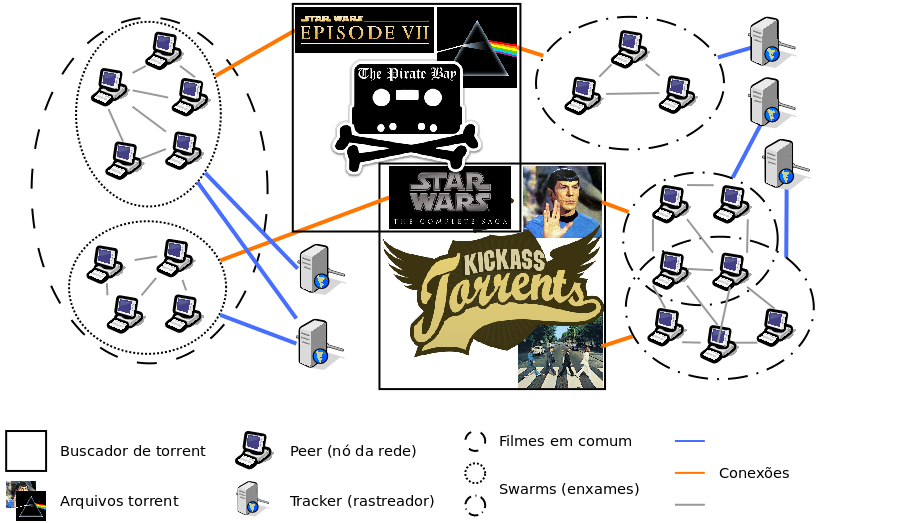
\includegraphics[width=\textwidth]{universobt.png}
                %\caption{Exemplo de grafo $G_i$.}
                %\label{fig:Gi}
              \end{figure}
            \end{block}

            \blockouterspace

            \begin{block}{Funcionamento do BitTorrent}
              \begin{columns}[t,\textwidth]
                \begin{column}{.46\textwidth}
                  \justifying
                  \blindtext
                  \blindtext
                \end{column}

                \begin{column}{.46\textwidth}
                  \justifying
                  \blindtext
                  \blindtext
                \end{column}
              \end{columns}
            \end{block}
          }
        \end{minipage}
      \end{beamercolorbox}
    \end{column}
    % ---------------------------------------------------------%
    % end the column

    % ---------------------------------------------------------%
    % Set up a column
    \begin{column}{.24\textwidth}
      \begin{beamercolorbox}[center,wd=\textwidth]{postercolumn}
        \begin{minipage}[T]{.95\textwidth}  % tweaks the width, makes a new \textwidth
          \parbox[t][\columnheight]{\textwidth}{ % must be some better way to set the the height, width and textwidth simultaneously
            % Since all columns are the same length, it is all nice and tidy.  You have to get the height empirically
            % ---------------------------------------------------------%
            % fill each column with content

            \begin{block}{Anatomia}
              \begin{innercol}
                \blindenumerate[10]
              \end{innercol}
            \end{block}

            \blockouterspace

            \begin{block}{Simulação}
              \begin{innercol}
                \begin{figure}[H]
                  \newlength{\myvsize}
                  \newlength{\myhsize}
                  \setlength{\myvsize}{4mm}
                  \setlength{\myhsize}{.3\textwidth}

                  \centering

                  \begin{subfigure}[H]{\myhsize}
                    \fbox{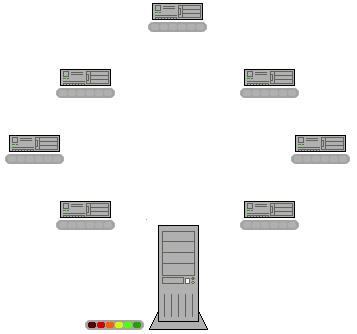
\includegraphics[width=\textwidth]{Torrentcomp_small-0.png}}
                    \caption{}
                    \label{fig:torrent-repr-0}
                  \end{subfigure}%
                  \quad %add desired spacing between images (~, \quad, \qquad or blank line)
                  \begin{subfigure}[H]{\myhsize}
                    \fbox{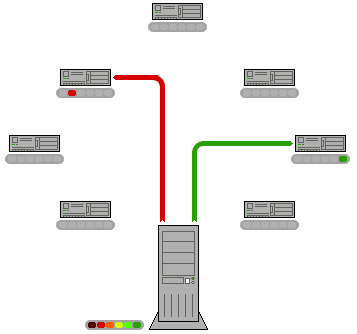
\includegraphics[width=\textwidth]{Torrentcomp_small-1.png}}
                    \caption{}
                    \label{fig:torrent-repr-1}
                  \end{subfigure}%
                  \quad
                  \begin{subfigure}[H]{\myhsize}
                    \fbox{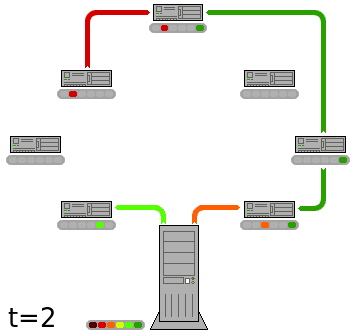
\includegraphics[width=\textwidth]{Torrentcomp_small-2.png}}
                    \caption{}
                    \label{fig:torrent-repr-2}
                  \end{subfigure}

                  \vspace{\myvsize}

                  \begin{subfigure}[H]{\myhsize}
                    \fbox{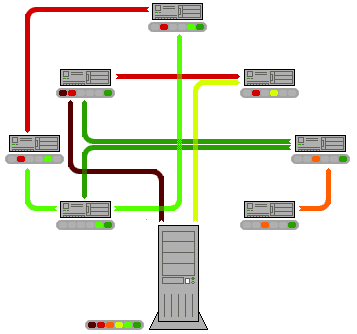
\includegraphics[width=\textwidth]{Torrentcomp_small-3.png}}
                    \caption{}
                    \label{fig:torrent-repr-3}
                  \end{subfigure}%
                  \quad
                  \begin{subfigure}[H]{\myhsize}
                    \fbox{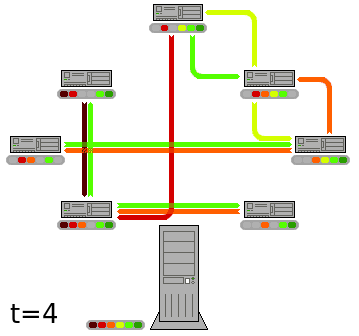
\includegraphics[width=\textwidth]{Torrentcomp_small-4.png}}
                    \caption{}
                    \label{fig:torrent-repr-4}
                  \end{subfigure}%
                  \quad
                  \begin{subfigure}[H]{\myhsize}
                  \fbox{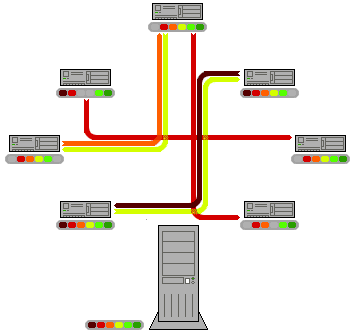
\includegraphics[width=\textwidth]{Torrentcomp_small-5.png}}
                  \caption{}
                  \label{fig:torrent-repr-5}
                  \end{subfigure}

                  \vspace{\myvsize}

                  \begin{subfigure}[H]{\myhsize}
                    \fbox{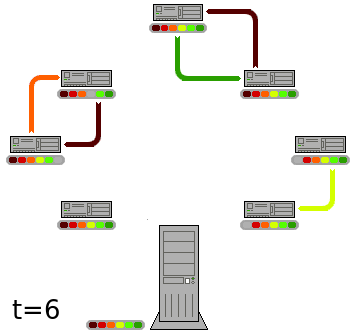
\includegraphics[width=\textwidth]{Torrentcomp_small-6.png}}
                    \caption{}
                    \label{fig:torrent-repr-6}
                  \end{subfigure}%
                  \quad
                  \begin{subfigure}[H]{\myhsize}
                    \fbox{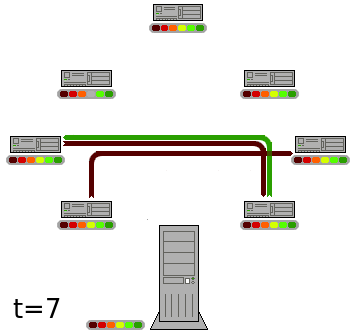
\includegraphics[width=\textwidth]{Torrentcomp_small-7.png}}
                    \caption{}
                    \label{fig:torrent-repr-7}
                  \end{subfigure}%
                  \quad
                  \begin{subfigure}[H]{\myhsize}
                    \fbox{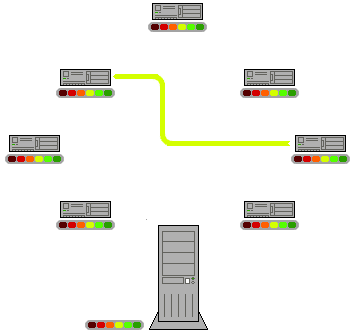
\includegraphics[width=\textwidth]{Torrentcomp_small-8.png}}
                    \caption{}
                    \label{fig:torrent-repr-8}
                  \end{subfigure}

                  \vspace{\myvsize}

                  \begin{subfigure}[H]{\myhsize}
                    \fbox{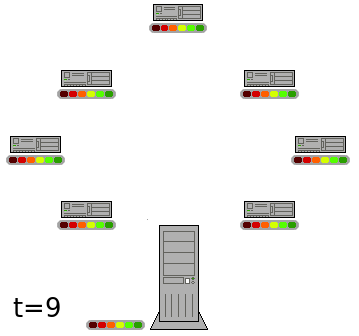
\includegraphics[width=\textwidth]{Torrentcomp_small-9.png}}
                    \caption{}
                    \label{fig:torrent-repr-9}
                  \end{subfigure}
                \end{figure}
              \end{innercol}
            \end{block}

            \blockouterspace

            \begin{block}{Referências}
             \begin{columns}
                \hspace{-2.5ex}
                \begin{column}{.97\textwidth}
                  \justifying
                  \scriptsize{
                    \begin{thebibliography}{99}
                      \bibitem{sandvine}
                        Sandvine Inc.
                        \textbf{Global Internet Phenomena Report --- 1H 2013}, 2013. \\
                        \url{http://macaubas.com/wp-content/uploads/2013/05/Sandvine_Global_Internet_Phenomena_Report_1H_2013.pdf}

                      \bibitem{torrentfreak:twitter}
                        Ernesto.
                        \textbf{BitTorrent Makes Twitter’s Server Deployment 75x Faster},
                        16 de julho de 2013. \emph{TorrentFreak}\\
                        \url{http://torrentfreak.com/bittorrent-makes-twitters-server-deployment-75-faster-100716/}

                      \bibitem{torrentfreak:facebook}
                        Ernesto.
                        \textbf{Facebook Uses BitTorrent, and They Love It},
                        25 de junho de 2013. \emph{TorrentFreak}\\
                        \url{http://torrentfreak.com/facebook-uses-bittorrent-and-they-love-it-100625/}

                      \bibitem{wiki:timeline}
                        Wikipedia.
                        \textbf{Timeline of file sharing} --- \emph{Wikipedia{,} The
                        Free Encyclopedia}, 2013.
                        \url{http://en.wikipedia.org/wiki/Timeline_of_file_sharing}

                      \bibitem{swarming}
                        Matheus B. Lehmann, Rodrigo B. Mansilha, Marinho P. Barcellos e
                        Flávio Roberto Santos.
                        \textbf{``Swarming: como BitTorrent revolucionou a Internet''}.
                        Em \emph{Atualizações em Informática}. PUC-Rio. Vol. 1. Rio de
                        Janeiro, 2011. Cap. 6, pp. 209–258
                    \end{thebibliography}
                  }
                \end{column}
              \end{columns}
            \end{block}
          }
        \end{minipage}
      \end{beamercolorbox}
    \end{column}
    % ---------------------------------------------------------%
    % end the column

  \end{columns}
  \vskip1ex
  %\tiny\hfill\textcolor{ta2gray}{Created with \LaTeX \texttt{beamerposter}  \url{http://www-i6.informatik.rwth-aachen.de/~dreuw/latexbeamerposter.php}}
  \tiny\hfill{Created with \LaTeX \texttt{beamerposter}  \url{http://www-i6.informatik.rwth-aachen.de/~dreuw/latexbeamerposter.php} \hskip1em}
\end{frame}
\end{document}

%%%%%%%%%%%%%%%%%%%%%%%%%%%%%%%%%%%%%%%%%%%%%%%%%%%%%%%%%%%%%%%%%%%%%%%%%%%%%%%%%%%%%%%%%%%%%%%%%%%%
%%% Local Variables:
%%% mode: latex
%%% TeX-PDF-mode: t
%%% End: